\documentclass{article}[11pt]

\newcommand{\bad}[1]{\emph{\textcolor{red}{#1}}}

\usepackage{amsthm}
\usepackage{amssymb}
\usepackage{amsmath}
\usepackage{mathtools}

\usepackage{epigraph}

\DeclareMathOperator{\img}{Im}
\DeclareMathOperator{\polylog}{\text{polylog}}
\DeclareMathOperator{\st}{\text{ such that }}

\newcommand{\contr}[0]{ $\Rightarrow\!\Leftarrow$ }
\newcommand{\defeq}{\vcentcolon=}
\newcommand{\eqdef}{=\vcentcolon}

\newtheorem{fact}{Fact}
\newtheorem{definition}{Definition}
\newtheorem{remark}{Remark}
\newtheorem{proposition}{Proposition}
\newtheorem{lemma}{Lemma}
\newtheorem{corollary}{Corollary}
\newtheorem{theorem}{Theorem}

\usepackage{tcolorbox}
\newenvironment{lem}[1][Lemma] { \begin{tcolorbox}[colback=green!10,coltitle=green!20!black,colframe=green!25,title=#1] } { \end{tcolorbox} }
\newenvironment{cor}[1][Corollary] { \begin{tcolorbox}[colback=green!10,coltitle=green!20!black,colframe=green!25,title=#1] } { \end{tcolorbox} }
\newenvironment{prop}[1][Proposition] { \begin{tcolorbox}[colback=green!10,coltitle=green!20!black,colframe=green!25,title=#1] } { \end{tcolorbox} }
\newenvironment{defn}[1][Definition] { \begin{tcolorbox}[colback=orange!10,coltitle=orange!20!black,colframe=orange!25,title=#1] } { \end{tcolorbox} }
\newenvironment{fct}[1][Fact] { \begin{tcolorbox}[colback=orange!10,coltitle=orange!20!black,colframe=orange!25,title=#1] } { \end{tcolorbox} }
\newenvironment{rmk}[1][Remark] { \begin{tcolorbox}[colback=orange!10,coltitle=orange!20!black,colframe=orange!25,title=#1] } { \end{tcolorbox} }
\newenvironment{thm}[1][Theorem] { \begin{tcolorbox}[colback=blue!10,coltitle=blue!20!black,colframe=blue!25,title=#1] } { \end{tcolorbox} }
\newenvironment{pf}[1][Proof] { \begin{tcolorbox}[colback=red!10,coltitle=red!20!black,colframe=red!25,title=#1] } { \end{tcolorbox} }

\title{The FUNDAMENTAL THEOREM OF CALCULUS} 
\author{Alek Westover}

\begin{document}
\maketitle
\tableofcontents

\section{The derivative in $\mathbb{R}$}
The derivative of a function $f (a,b) \to \mathbb{R}$\footnote{You might ask why I chose $(a,b)$ as the domain for $f$. You might also ask what $a, b$ are. Well, $a,b$ are extended real numbers (real numbers or $\pm \infty$). And I chose this interval because open balls form a basis for the topology on $\mathbb{R}$ that we are using. So yeah.} at a point $x$ is defined as 
$$f'(x) \defeq \lim_{h\to 0} \frac{f(x+h)-f(x)}{h}.$$
This can be interpreted geometrically as the slope of the tangent line to a curve\footnote{
But what is the definition of $\lim_{h\to 0}$ you might ask. Also does this even exist you might ask. A function is called differentiable if the limit exists. The formal definition of the limit is $$\lim_{h\to 0}g(h) = L \iff \forall \epsilon > 0 \exists \delta > 0 \st |h| < \delta \implies |g(h)-L| < \epsilon.$$ }.
It can also be interpreted as the rate of change of the function. This is nice because this reflects clearly the "$1$-dimensional nature" of the opperator.

\section{The integral in $\mathbb{R}$}
The integral is defined as 
\begin{multline*}
\int_{a}^{b}f(x) dx \defeq \lim_{n\to\infty} \sum_{k=1}^n \frac{b-a}{n} f(x_k), \\
\text{for any $x_k$ satisfying $x_k-a\in\Big[\frac{b-a}{n}(k-1), \frac{b-a}{n}k\Big]$}.
\end{multline*}

This can be interpreted geometrically as the signed area between a graph and the axis\footnote{Note that $$\lim_{n\to\infty}f(n) = L \iff \forall \epsilon>0 \exists M \st \forall m>M, |f(m)-L| < \epsilon.$$
	If you interpret $f$ as a density function, the integral can be interpreted physically as the mass of the line segment from $[a, b]$. This is kind of nice because its very clearly $1$-dimensional.
Also note that the some restrictions must be imposed in order to ensure that this is well defined, and a convergent sum. 
To analyze the convergence of the sum it is useful to consider the "upper" and "lower" sums (the sums you get when you take the supremum/infimum of the values of $f(x)$ over all valid choices of $x_k$ to be the value that you use in the sum) because these give an upper and lower bound for the integral.
If the upper and lower sums agree, then the function is said to be integrable, and its integral is either of the sums.
}.

\section{Fundamental Theorem of Calculus}
\begin{theorem}[Fundamental Theorem of Calculus]
	\label{thm:FTC}
	If $f : [a, b] \to \mathbb{R}$ is a continuous function with integrable derrivative, then 
	$$\int_{a}^{b} f'(x) dx = f(b) - f(a).$$
\end{theorem}
To prove this we must first establish the following theorem:
\begin{theorem}[Mean Value Theorem]
	\label{thm:MVT}
	If $f : [a, b] \to \mathbb{R}$ is a continuous, differentiable\footnote{Note that this is redundant, differentiability implies continuity} function, then 
	$$\exists c\in (a, b) \st f'(c) = \frac{f(b) - f(a)}{b - a}.$$
\end{theorem}
To prove this we must first establish the following theorem:
\begin{theorem}[Rolle's Theorem]
	\label{thm:rolle}
	If $f : [a, b] \to \mathbb{R}$ is a continuous, differentiable function with $f(a) = f(b)$, then 
	$$\exists c\in (a, b) \st f'(c) = 0.$$
\end{theorem}
To prove this we must first establish the following lemma and 2 theorems:
\begin{lemma}[Derivative at Extrema is $0$]
	\label{lem:derivAtExtrema}
	Let $f(x) : [a,b] \to \mathbb{R}$	be a continuous, differentiable function with a maximum at some $c\in (a,b)$. Then 
	$$f'(c) = 0.$$
\end{lemma}
\begin{lemma}[Intermediate Value Theorem]
	\label{lem:IVT}
	If $f : [a,b] \to \mathbb{R}$ is a continuous function such that $f(a) < f(b)$, and if $k \in (f(a), f(b))$, then 
	$$\exists c\in (a, b) \st f(c) = k.$$
\end{lemma}
\begin{theorem}[Extreme Value Theorem]
	\label{thm:extremeValue}
	If $f: [a,b] \to \mathbb{R}$ is a continuous function, then 
	$$f \text{ achieves extrema on } [a, b].$$
\end{theorem}
To prove this we must first establish the following theorem: 
\begin{theorem}[Bolzano-Weierstrass Theorem]
	\label{thm:bolzanoWeierstrass}
	If $\{x_i\}_{i=0}^\infty$ is a bounded infinite sequence of values in $[a,b]$\footnote{Really any compact space, I'm just using [a,b] because this is the version that we need for the proof of the version of the extreme value theorem that we need for the proof of rolles theorem that we need for the proof of the mean value theorem that we need for the proof of the FUNDAMENTAL THEOREM OF CALCULUS.}, then there is  a convergent subsequence of the sequence.
\end{theorem}

To do this we need the following lemma.
\begin{lemma}[A closed interval contains all its limit points]
	\label{lem:intervalContainsLimitPts}
	Let $\{x_i\}_{i=1}^\infty$ be a sequence of values in $[a,b]$ that converges to some value in $\mathbb{R}$. 
	Then $$\lim_{i\to \infty} x_i \in [a, b].$$
\end{lemma}

This might be kind of confusing, so see Figure \ref{fig:flowchart} below for the dependency tree.
\begin{center}
	\begin{figure}[h]
		\label{fig:flowchart}
	\centering
	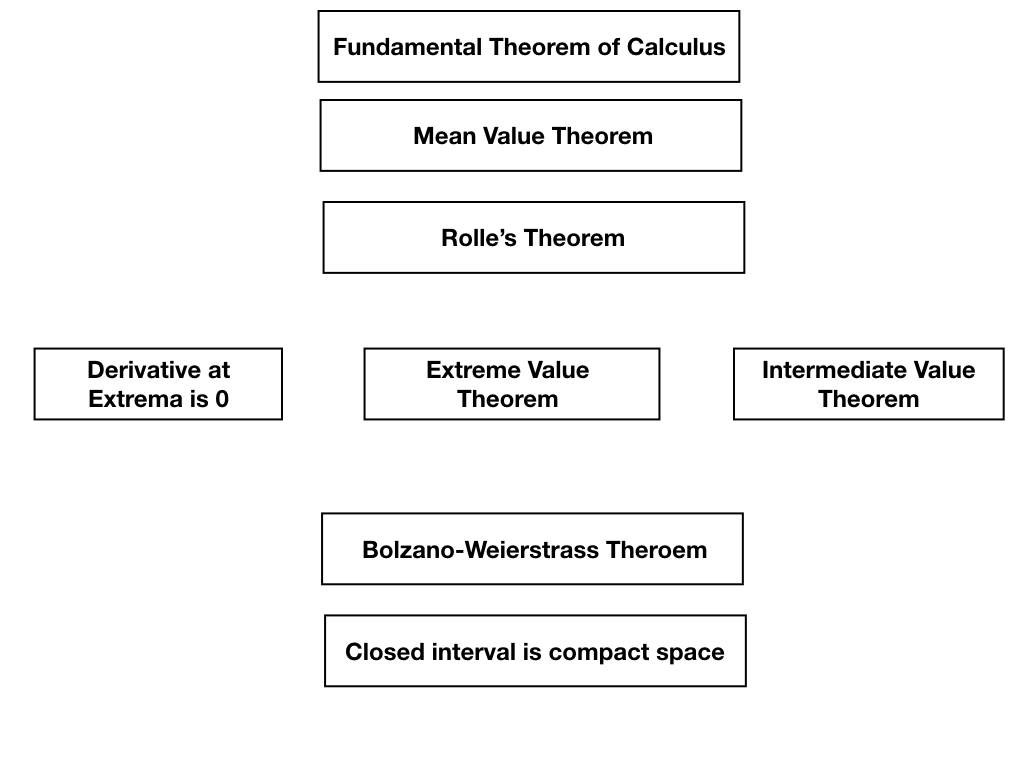
\includegraphics[width=\linewidth]{ftcFlowChart/ftcFlowChart.png}
	\caption{pretty gnarly flowchart}
\end{figure}
\end{center}

\epigraph{Enough talk. Lets fight!}{Po}

\begin{proof}[Proof of Lemma \ref{lem:intervalContainsLimitPts}]{Closed Interval Contains Limit Points}
	Let $x$ be the value that the sequence converges to. 
	By the definition of a limit, 
	$$\forall \epsilon > 0 \exists M>0 \st \forall i>M, |x-x_i|< \epsilon.$$

	Assume for contradiction that $x\not\in [a,b]$. 
	WLOG let $x>b$. But then if we set $\epsilon = (x-b)/2$,
	$$\exists M>0 \st \forall i>M, |x-x_i| < (x-b)/2.$$
	Rearanging the inequality, 
	$$ x-\frac{x-b}{2}< x_i < x+\frac{x-b}{2}.$$
	But then
	$$ b < \frac{x+b}{2}< x_i < \frac{3x-b}{2}.$$
	This contradicts the fact that all $x_i \in [a, b].$\contr
\end{proof}


\begin{proof}[Proof of Theorem \ref{thm:bolzanoWeierstrass}]{Bolzano-Weierstrass Theorem}
	First we prove the following claim: $$\text{Every infinite sequence has a monotonic subsequence}.$$
	We consider $2$ cases. 
	\paragraph{Case 1: There are infinitely many terms in the sequence that are greater than all later terms.} That is, there are infinitely many $n$ such that $x_n > x_m$ for all $m> n$. In this case we can take the sequence formed by successively taking these "dominant" terms, and this sequence will clearly be monotonically decreasing.
	\paragraph{Case 2: There are finitely many terms in the sequence that are greater than all later terms.} That is, $$\exists N, \st \forall n \ge N, \exists m \st x_n < x_m.$$ 
	In this case we can create a monotonically increasing sequence as follows: take $x_N$ as the first term in the sequence, and then to get the $(n+1)$-th term in the sequence from the $n$-th, take $m$ such that $x_m$ is greater than the $n$-th term (this must exist by hypothesis) and use $x_m$ as the $(n+1)$-th term in the seqence.\\
	Now it is sufficient to show that a bounded monotonic sequence converges. \\
	WLOG we consider a monotonically increasing sequence (a monotonically decreasing sequence could be negated to achieve a monotonically increasing sequence, so by negating twice this result holds for monotonically decreasing sequences too). Then consider $$s = \sup{\{x_i\}_{i=0}^\infty}.$$ 
	Clearly this exists because the sequence is bounded.
Note that by definition of the supremum\footnote{It occurs to me that I probably have not defined the supremum. Here is the definition in words: the supremum of a set is the least upper bound for the set.}, 
	$$\forall \epsilon > 0, \exists n \st s-x_n < \epsilon.$$
	(Because if this were not so then we could find a smaller lower bound than the supremum which is a contradiction).
	But in the case of a monotonically increasing seqeunce this actually implies:
	$$s-x_n < \epsilon \implies s-x_m < \epsilon, \forall m \ge n.$$
	So, we have that 
	$$\forall \epsilon > 0, \exists n \st \forall m \ge n, |s-x_n| < \epsilon.$$
	That is, the sequence converges.
	Thus, we have the result that all bounded sequences have convergent subsequences.
\end{proof}

\begin{proof}[Proof of Theorem \ref{thm:extremeValue}]{Extreme Value Theorem}
	We need only establish that all such functions achieve a maxima, and then the dual property of a minima being achieved is immediate by considering the negated function.
We first establish that a continuous function on a closed interval is bounded\footnote{You might be wondering "did you ever define continuity?". I don't know. So here is a definition: A function $f$ is continuous at a point $x$ if and only if $\forall \epsilon > 0, \exists \delta \st \forall $y$ \st |x-y|<\delta, |f(x)-f(y)|<\epsilon$.}.

Assume the contrary. 
Then there must be a sequence of values in $[a,b]$, say $\{x_n\}_{n=1}^\infty \st f(x_n) > n, \forall n$.
Because we have a bounded sequence, we the Bolzano-Weierstrass Theorem tells us that there must be some convergent subsequence, say $\{x_{n_k}\}_{k=1}^\infty$ that converges to some value. 
By Lemma \ref{lem:intervalContainsLimitPts}, we know that the point that the sequence converges to must lie in $[a,b]$. Call this point $\alpha$.
Now, note that because $f$ is a continuous function on $[a,b]$, in particular $f$ is continuous at $\alpha$, that is:
$$\forall \epsilon > 0, \exists \delta \st |x-\alpha| < \delta \implies |f(x)-f(\alpha)| < \epsilon.$$
Take some $\epsilon > 0$. For all $\delta > 0, \exists N \st \forall n_k > N, |x_{n_k} - \alpha| < \delta$ because the sequence converges to $\alpha$.
But, $f(x_{n_k}) > n_k$, so $\exists n_k > N \st f(x_{n_k}) - f(\alpha) \ge \epsilon$.
This contradicts the continuity of $f$ at $\alpha$.
Thus we have established that a continuous function on a closed interval must be bounded\footnote{Note that if the interval were open but finite, the point of convergence generated by Bolzano-Weierstrass may have not been in the domain of the function, which would wreck the proof, and if the interval were unbounded then Bolzano-Weierstrass wouldn't have applied, so we really do need these conditions (there are lots of easy counterexamples to show this as well, think about what happens if you try to find the minima of $1/x$ on $\mathbb{R}^+$ or try to find the maxima of $1/x$ on $(0,1]$).}.

Let $M = \sup{\{f(x) : x \in [a, b]\}}$. We now aim to show that $M$, which exists because the function is bounded, is actually achieved. 
We know that by the definition of the supremum, 
$$\forall \epsilon > 0, \exists x\in [a,b] \st M-f(x) < \epsilon.$$
Form a sequence of $x_n$ satisfying $M-f(x_n) < \frac{1}{n}$.
Take a convergent subsequence $x_{n_k}$ of the sequence. 
Let the value that the subsequence converges to be $\alpha$. 
Note that $\alpha \in [a, b]$.
Then, because $f$ is continuous at $\alpha$, if we take some $\epsilon > 0$, 
$$ \exists \delta > 0 \st |x-\alpha| < \delta \implies |f(x) - f(\alpha)| < \epsilon.$$
By the convergence of the subsequence, $\exists N \st \forall n_k > N, |x_{n_k}  - \alpha| < \delta.$
Thus $|f(x_{n_k}) - f(\alpha)| < \epsilon, \forall n_k > N$.
Recall that $f(x_{n_k}) > M - 1/n_k$.
Thus, 
$f(\alpha) > M - \epsilon - 1/n_k$.
But the only value of $f(\alpha)$ that satisfies this for all values of $\epsilon$ and $n_k$ is $M$, so $f(\alpha) = M$.

\end{proof}

\begin{proof}[Proof of \ref{lem:derivAtExtrema}]{(Derivative at Extrema is 0)}
	WLOG say that the extrema is a maxima\footnote{Note: I love using the duality of min/max or inf/sup under negation (i.e. reversing set orderings)!}.

	We proceed by contradiction, i.e. by assuming that $f'(c) \neq 0$. There are $2$ cases.
	\paragraph{Case: $f'(c) > 0$}
	By an interpretation of the definition of the derivative's defining limit,\footnote{Note that by assumption the limit (i.e. derivative exists). Also note that we can have $h\to 0$ using any sequence that converges to $0$. I chose the sequence $(1/n)_{n=1}^{\infty}$ here, but could have just as well have chosen $(1/n^2)_{n=1}^{\infty}$. Because the limit exists these all give the same value for the derivative.}. 
	$$\forall \epsilon > 0, \exists N \st \forall n>N, \Big|\frac{f(c+\frac{1}{n}) - f(c)}{\frac{1}{n}} - f'(c)\Big| < \epsilon.$$
	We can set $\epsilon = \frac{1}{2}f'(c) > 0$. 
	This implies:
	$$0< \frac{1}{2}f'(c) \frac{f(c+\frac{1}{n}) - f(c)}{\frac{1}{n}} < \frac{3}{2} f'(c).$$
	But then $f(c+\frac{1}{n})> f(c)$, which is not possible because $f(c)$ is a maxima.
	\paragraph{Case: $f'(c) < 0$}
	Now we will use an alternate definition of the derivative:\footnote{Note that the sequences I chose in this and the previous paragraph effectively implement approaching from below and approaching from above according to a nice regular path.}
	$$\forall \epsilon > 0, \exists N \st \forall n>N, \Big|\frac{f(c-\frac{1}{n}) - f(c)}{-\frac{1}{n}} - f'(c)\Big| < \epsilon.$$
	We set $\epsilon = -\frac{1}{2}f'(c) > 0$. 
	This implies:
	$$\frac{3}{2}f'(c) \frac{f(c-\frac{1}{n}) - f(c)}{-\frac{1}{n}} < \frac{1}{2} f'(c) < 0.$$
	But then $f(c-\frac{1}{n}) > f(c)$, which is not possible because $f(c)$ is a maxima.\\
	
	We have shown that assuming either $f'(c) < 0$ or assuming $f'(c) > 0$ leads to a contradiction. Thus $0 \le f'(c) \le 0$, i.e. $f'(c) = 0$.
\end{proof}

\begin{proof}[Proof of Theorem \ref{lem:IVT}]{Intermediate Value Theorem}
	Consider $\{x \in [a, b] : f(x) < k \}$. 
	Let $s = \sup \{x \in [a, b] : f(x) < k \}$. 
	I claim that $f(s) = k$. 
	First of all note that $f(s) \ge k$. This is easily shown by contradiction: if $f(s) < k$ then by the continuity of $f$ at $s$, if we consider the open ball of radius $\frac{k - f(s)}{2}$ around $f(s)$, then the preimage of this ball consists of points $x$ that all satisfy $f(x) < k$, but some of these points have $x>s$	(note that it is possible that some points in this ball are not in $[a,b]$, but $s \neq b$, so there is at least one point $x \in [a,b]$ in this ball with $x > s$) which contradicts the fact that $s$ is the supremum.
	Now, by the definition of the supremum, 
	$$\forall x \in (a, s), \exists y \in [a,b] \st f(y) < k, y > x.$$
Then, consider the sequence $x_n$ defined as follows: to get $x_n$ let $x=\max(a, s-\frac{1}{n})$\footnote{Note the slightly annoying fact that $s-\frac{1}{n}$ might not be in $[a,b]$, but this is easily fixable as $\max(a, s-\frac{1}{n})$ is definitely in the interval. Also, after a while the $\max$ condition is not necessary, because $s-\frac{1}{n}>a$ for some $n$}, and then take $x_n \in [a, b] \st x_n > x, f(x_n) < k$ which is guaranteed to exist. 
This sequence $x_n$ satisfies $f(x_n) < k$ for all $k$, and also, as shown before, a continuous function on a closed interval must be bounded, so $f(x_n)$ is a sequence with values in $[-M, k)$ for some $M$, so $f(x_n)$, which must converge because $x_n$ is continuous, converges to a value in $[-M, k]$ (the closure of the set that its values are in). Because the sequence $x_n$ converges to $s$, we have that $f(s) \le k$.
Now, 
$$k \le f(s) \le k\implies f(s) = k.$$
\end{proof} 

\begin{proof}[Proof of Theorem \ref{thm:rolle}]{Rolle's Theorem}
	Firstly, note that if $f$ is a constant function, then the result is trivially true.
	Now, consider a non-constant function $f$. By the Extreme Value Theorem it achieves a maxima somehwere, and by the fact that extrema implies derivative is $0$, we know that there is some point where the derivative is $0$.
\end{proof}

\begin{proof}[Proof of Theorem \ref{thm:MVT}]{Mean Value Theorem}
	Consider the funciton $$L(x) = \frac{f(b)-f(a)}{b-a}(x-a)+f(a).$$
	Note that $L(a) = f(a), L(b) = f(b).$
	Now consider the function $g(x) = f(x) - L(x).$
	Note that $g(a) = g(b) = 0.$
	All the hypothesis for Rolle's theorem apply. Thus $\exists c \in [a,b ] \st g'(c) = 0$.
	But $g'(x) $ is simply, by linearity of the derivative,
	$$g'(x) = f'(x) - \frac{f(b)-f(a)}{b-a}.$$
	Thus
	$$g'(c) = 0 = f'(c) - \frac{f(b)-f(a)}{b-a} \implies f'(c) = \frac{f(b)-f(a)}{b-a}.$$
\end{proof}

\begin{proof}[Proof of Theorem \ref{thm:FTC}]{THE FUNDAMENTAL THEOREM OF CALCULUS}
	Consider the expression of $f(b)-f(a)$ as a telescoping sum\footnote{One might well ask, "what is the motivation behind doing this?" The motivation is the awesomeness of the mean value theorem.}:
	$$f(b)-f(a) = \sum_{i=1}^n f\Big(a + \frac{i\cdot(b-a)}{n}\Big)-f\Big(a+\frac{(i-1)\cdot(b-a)}{n}\Big).$$
	Taking the limit as $n\to \infty$ of both sides cannot change the equality because neither side ultimately depends on $n$.\footnote{Another way (possibly more rigorous) of seeing why taking limits is valid is to note that for any $n$, the sum is $f(b) - f(a)$, so really $\forall \epsilon > 0, \exists N = 1, \st \forall n>N,$ $$\Big|\sum_{i=1}^n f\Big(a + \frac{i\cdot(b-a)}{n}\Big)-f\Big(a+\frac{(i-1)\cdot(b-a)}{n}\Big) - (f(b) - f(a))\Big| = 0 < \epsilon.$$}
	$$\lim_{n\to\infty}f(b)-f(a) = \lim_{n\to\infty}\sum_{i=1}^n f\Big(a + \frac{i\cdot(b-a)}{n}\Big)-f\Big(a+\frac{(i-1)\cdot(b-a)}{n}\Big).$$
	Now we apply the Mean Value Theorem to each interval $\Big(a + \frac{i\cdot(b-a)}{n},a+\frac{(i-1)\cdot(b-a)}{n}\Big)$, which yields
	$$f(b)-f(a) = \lim_{n\to\infty} \sum_{i=1}^\infty \frac{b-a}{n}f'(x_k)$$
	for some $x_k$ in the appropriate interval.
	This is the definition of the integral of $f'$, i.e. 
	$$f(b) - f(a) = \int_a^b f'(x) dx.$$
	\Huge{Q.E.D.}
\end{proof}

\section{Vector fields}
A vector field\footnote{for our purposes here today} is a function $f: \mathbb{R}^2 \to \mathbb{R}^2$.
This can be interpreted geometrically as assigning to every point in the plane a vector.

\section{Parametric Functions}
A parametric function\footnote{for our purposes here today} is a function $\gamma : \mathbb{R} \to \mathbb{R}^2$.
This can be interpretted geometrically as a correspondence between time and position, i.e. at any time $t$, $\gamma(t)$ specifies the position of the object.

\section{Integrals over regions in $\mathbb{R}^2$ }
The integral of some function $f(x, y)$ over a region $ D \subset \mathbb{R}^2$ is defined to be 
$$\int_D f(x,y) dx dy \defeq \sum_{\text{rect}_i \in \text{ all rects}}f(x_i, y_i) \cdot \text { area of rect}_i.$$
This can be interpreted geometrically as the signed volume between a surface in $\mathbb{R}^3$ and the $xy$-plane.
It can be interpreted physically as the mass of something when $f$ is a density.
Note that this can be separated into $2$ single integrals in $2$ ways, that turn out to be equivalent by Fubini's Theorem.

\section{Line integrals in $\mathbb{R}^2$}
Work is a physicsy thing. 
Line integrals look kinda like
$$\int_C \vec{F}(\vec{\gamma}(t))\cdot \vec{\gamma}'(t) dt$$
They represent work.
Note that there is no "new definition" here, this is just a single variable integral (albiet a potentially complicated one).
What's that derrivative thing?
Well note that $\gamma : \mathbb{R} \to \mathbb{R}^2$ such that 
$$t \mapsto \begin{bmatrix} \gamma_x(t) \\ \gamma_y(t) \end{bmatrix}.$$
Then,
$$\gamma'(t) \defeq \begin{bmatrix} \gamma_x'(t) \\ \gamma_y'(t) \end{bmatrix}.$$


\section{Green's theorem}
\begin{theorem}[Green's theorem]
	\label{thm:green}
	Let $S\subset \mathbb{R}^2$, and let $f, g : S \to \mathbb{R}$
	$$\int_{\partial S} f dx + g dy = \int_{S} \frac{dg}{dx} - \frac{df}{dy} dx dy.$$
\end{theorem}

\begin{proof}
	First we will show that it is true for a square. Then we will piece together squares, like in the motivation behing the definition of the integral, and we will discover that stuff on the boundary cancels, which yields the formula.\\
	For the square: explicitely compute the line integral, parameterize each side separately. You'll need the mean value theorem to do this. You'll get $h^2(\frac{dg}{dx} - \frac{df}{dy})$ where those derivatives are evaluated somewhere on the square. But the square is small, so how wrong could it possibly be?\\
	When you have adjacent squares the integrals add, and the shared side cancels.
\end{proof}

\begin{corollary}[Area from line integral]
Let $S\subset \mathbb{R}^2$, then 
$$[S] = \int_S dx dy = \frac{1}{2}\int_{\partial S} -ydx + xdy.$$
\end{corollary}
\begin{proof}
	This is trivial from Theorem \ref{thm:green}: simply verify that the exterior derrivative of $xdy-ydx$ is $dx \wedge dy$.
\end{proof}
This is kinda awesome (imo) because it means that knowing the funciton on the boundary (and that the function is well-behaved, i.e. continuous, differentiable, that stuff) tells you about the area.

\end{document}

